% CAP 3
\chapter{Estado del Arte}

De los trabajos que existen en la actualidad, podemos mencionar tres que resultan de especial interés, ya que los enfoques y las propuestas de solución que emplean son un reflejo de cómo se ha estado abordando la problemática y como se ha tratado de resolver. 

\section{Cellular Automata Automatically Constructed from a Bioconvection Pattern}

Este trabajo \citep{kawaharada2016cellular} se centra en realizar el descubrimiento de las reglas de evolución para un autómata celular unidimensional a partir de los datos observados de los patrones de bioconvección generados como resultado de la respuesta a una estimulación luminosa de un tipo de alga unicelular llamada Euglena gracilis. Empleando métodos de análisis estadísticos para la obtención de estas reglas.
El proceso lo realizan de la siguiente forma:

\begin{enumerate}
	\item Recopilación de imágenes de los patrones de bioconvección.
	\item Transformación de las imágenes recopiladas a escala de grises.
	\item Uso de filtros para la eliminación del ruido.
	\item Discretización de las imágenes en escala de grises.
	\item Se predetermina el número de estados para el sitio $k$ y se discretiza la información observada acorde a esto.
	\item Basado en el número de vecinos establecido $m$ se calcula la frecuencia con la que aparecen los estados por cada combinación de posibles estados vecinos.
\end{enumerate}

\section{Discovery of Transition Rules for Cellular Automata Using Artificial Bee Colony and Particle Swarm Optimization Algorithms in Urban Growth Modeling}

En este trabajo \citep{naghibi2016discovery} se muestra un método para descubrir las reglas de transición de un autómata celular de lattice bidimensional que modele el crecimiento urbano empleando un algoritmo de optimización de colonia de abejas artificiales. Para ello utilizan como datos de entrada información multitemporal sensada remotamente de el área urbana de la ciudad de Urmia, Iran.
\\
\\
Otras técnicas que utilizan además de la colonia de abejas artificiales son:
\begin{itemize}
	\item Particle Swarm Optimization (PSO)
	\item Logistic Regression
\end{itemize}

\begin{figure}[h]
	\centering
	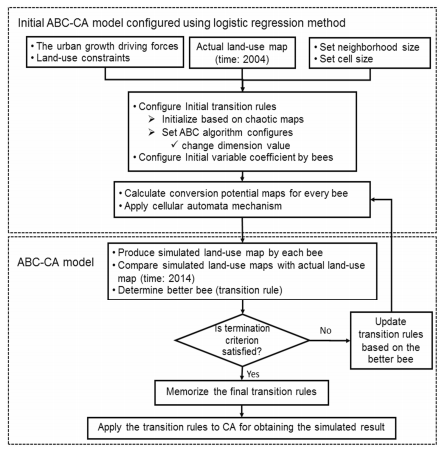
\includegraphics[width=\linewidth]{fig/abc}
	\caption{Modelo para la obtención de reglas del autómata celular empleando un algoritmo de optimización de colonia de abejas artificiales.}
	\label{fig:abc}
\end{figure}

\begin{figure}[h]
	\centering
	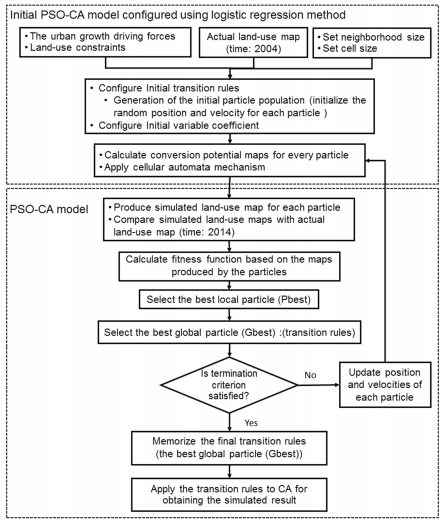
\includegraphics[width=\linewidth]{fig/pso}
	\caption{Modelo para la obtención de reglas del autómata celular empleando un algoritmo de optimización de enjambre de partículas.}
	\label{fig:pso}
\end{figure}

\begin{figure}[h]
	\centering
	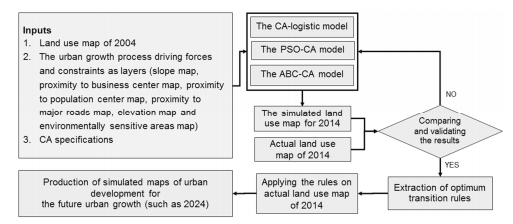
\includegraphics[width=\linewidth]{fig/evaluation}
	\caption{Modelo de evaluación de los algoritmos.}
	\label{fig:evaluation}
\end{figure}

\begin{figure}[h]
	\centering
	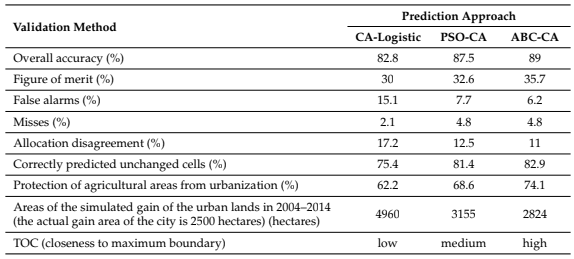
\includegraphics[width=\linewidth]{fig/results}
	\caption{Resultados de la evaluación de los algoritmos. }
	\label{fig:results}
\end{figure}

\section{On Routine Evolution of Complex Cellular Automata}

El enfoque de este trabajo \citep{bidlo2016routine} es la creación de un método para la obtención de un conjunto de reglas que puedan replicar un comportamiento, sin embargo no toman en cuenta conocimiento previo del fenómeno que se quiere replicar. Lo que se hace es utilizar un algoritmo evolutivo cuya función de aptitud es dependiente del resultado al que se quiere llegar y la codificación de las reglas viene dada de la siguiente forma:

\begin{figure}[h]
	\centering
	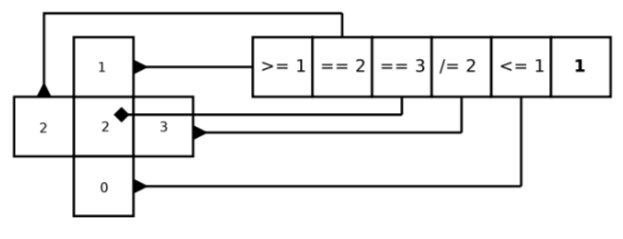
\includegraphics[width=\linewidth]{fig/rulesencoding}
	\caption{Ejemplo de la codificación de las reglas de evolución del autómata con un vecindario de tipo Moore.}
	\label{fig:results}
\end{figure}
